\chapter{Background Survey}\label{C:backgroundsurvey}
\section{Core Concepts}
A boolean formula is in Conjunctive Normal Form (CNF) if and only if it is a conjunction (and) of clauses. A clause in a CNF formula is given by a disjunction (or ) of literals. A literal is either an atom or the negation of an atom, an atom is one of the varables in the formula.\\

Consider the boolean formula $\lnot a \lor (b \land c)$, the CNF is $(\lnot a \lor b) \land (\lnot a \lor c)$. In this CNF formula the clauses are $(\lnot a \lor b)$, $(\lnot a \lor c)$, the literals used are $\lnot a$, $b$, $c$ and the atoms are $a$, $b$, $c$.\\

A boolean formula is in Disjunctive Normal Form (DNF) if and only if it is a disjunction (or) of clauses. A DNF clause is a conjunction (and) of literals. Literals and atoms are defined the same as in CNF formulas.\\

Consider the boolean formula $\lnot a \land (b \lor c)$, the DNF is $(\lnot a \land b) \lor (\lnot a \land c)$.\\


\section{Litrature Review}

A survey in 1995 focuses on rule extraction algorythms \cite{andrews1995survey}, identifying the reasons for needing these algorythms and introducing ways to categorise and compare them. Motivation behind scientific study is always crutial so why is understanding the knowledge contained inside Artificial Neural Networks's (ANN's) important? The key points indentified are that the ANN might of discovered some rule or patten in the data which is currently not known, being able to extract these rules would give humans a greater understanding of the problem. Another, prehapse more significant reason is the application of ANN's to systems which can effect the safty of human lives, i.e. Aroplanes, Cars. If using an ANN in the context of a system inboling human safty it is important to be certian of the knowledge inside the network, to be sure that the ANN wont take any dangourous actions.\\

There are three categories that rule extraction algorythms fall into \cite{andrews1995survey}. An algorythm in the \textbf{decompositional} category focuses on extracting rules from each hidden/output unit. If an algorythm is in the \textbf{pedagogical} category then rule extraction is thought of as a learning process, the ANN is treated as a black box and the algorythm learns a relationship between the input and output vectors. The third category, \textbf{electic}, is a combiniation of decompositional and pedagogical. Electic accounts for algorythms which inspect the hidden/output neurons individually but extracts rules which represent the ANN globally \cite{tickle1998truth}.\\

To further divide the categories two more classifications are introduced. One mesures the portability of rule extraction technequics, i.e. how easily can they be applyed to different types of ANN's. The second is criteria to assess the quallity of the extracted rules, these are accuracy, fidelity, consistency, comprehensibility \cite{andrews1995survey}.

\begin{enumerate}
\item A rule set is \textbf{Accurate} if it can generalize, i.e. classify previously unseen examples.
\item The behavour of a rule set with a high \textbf{fedelity} is close to that of the ANN it was extracted from.
\item A rule set is \textbf{consistent} if when trained under different conditions it generates rules which assign the same classifications to unseen examples.
\item The mesure of \textbf{comprehensibility} is defined by the numer of rules in the set and the number of literals per rule.
\end{enumerate}

The paper "Backpropagation for Neural DNF- and CNF-Networks" presents an approach which relies on a special NN archetechure. The neurons in these networks have a restricted functon space, they are only able to peform a OR or AND on a subset of their inputs. By restricting the degreese of freedom in the network it is possible to understand the actions each neuron is taking. Rules can simply be extracted from the trained network by inspecting these neurons \cite{herrmann1996backpropagation}. The conjunctive and disjunctive neurons presented, while making sense mathematically are combersom to implement. Insted a perfered way to implement logical neurons will be to use Noisy-OR and Noisy-AND neurons \cite{LearningLogicalActivations}. Noisy gates are derived from the Noisy-OR relation, developed by Judea Pearl \cite{russell1995modern}, a concept in Bayesian Networks. \\

A Bayesian Network represents the conditional dependencies between random variables in the form of a directed acyclic graph.

\begin{figure}[H]
  \centering
  \begin{minipage}[b]{0.4\textwidth}
    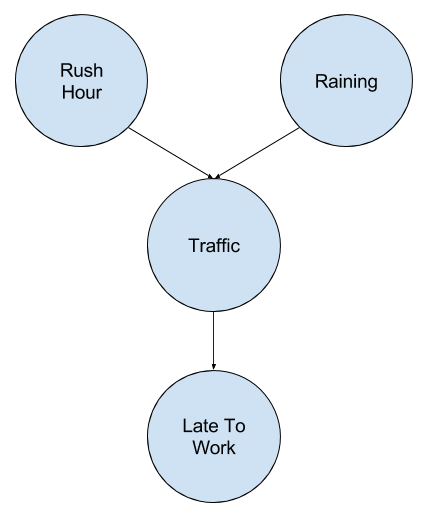
\includegraphics[width=\textwidth]{bayesian-network-example.png}
    \caption{}
    \label{fig:bayesian-network-example}
  \end{minipage}
  \hfill
\end{figure}

Figure \ref{fig:bayesian-network-example} is a Bayesian network, it demonstraits the dependency bettwen the random variables "Rush Hour", "Raining", "Trafic", "Late To Work". The connections show the dependencys i.e. Traffic influences whether you are late to work, and it being rush hour or raining influences whether there is trafic.\\

Consider a bayesian network, take some node $D$ with $S_1,..., S_n$ as parents where each $S_i$ is independent from all others, i.e. each $S_i$ influences the node $D$. The relationship between D and its parents is if $S_1\ OR\ ...\ OR\ S_n$ is true then $D$ is true. Let $\epsilon_i$ be the uncertanty that $S_i$ infludence $D$ then $P(D = 1| S_1, , S_n)$ can be defined.

\begin{align}
P(D = 1 | S_1, ..., S_n) = 1 - \prod^n_{i=1} \epsilon_i
\end{align}

In the context of a neuron, the inputs $x_1, ..., x_n$ represent the probability that inputs $1, ..., n$ are on. Each $\epsilon_i$ is the uncertanty as to whether $x_i$ infulences the output of the neuron. The definitions for Noisy-OR and Noisy-AND gates are given below

\begin{definition}
A \textbf{Noisy-OR} Neuron has weights $\epsilon_1, ..., \epsilon_n \in [0,1]$ which represent the irielevence of corosponding inputs $x_1, ..., x_n \in [0,1]$. The activation of a Noisy-OR Neurons is.

\begin{align}
a = 1 - \prod^p_{i=1} (\epsilon_i^{x_i}) \cdot \epsilon_b
\label{equ:noisy-or-activation-1}
\end{align}
\end{definition}

\begin{definition}
A \textbf{Noisy-AND} Neuron has weights $\epsilon_1, ..., \epsilon_n \in [0, 1]$ which represent the irielevence of corosponding inputs $x_1, ..., x_n \in [0,1]$. The activation of a Noisy-AND Neurons is.

\begin{align}
a = \prod^p_{i=1} (\epsilon_i^{1 - x_i}) \cdot \epsilon_b
\label{equ:noisy-or-activation-1}
\end{align}
\end{definition}

Both these paramatersations reduce to descrete logic gates when there is no noise, i.e. $\epsilon_i = 0$ for all $i$.\\

While the concept presented in \cite{herrmann1996backpropagation} is the foudation for the work presented in this report, the approach presented is different that what has been done. A different approach to disjunctive and conjunctive neurons is taken, along with this more investigation is carried out in terms of the capabilitys of these networks (when compared to a standard perceptron) and the rule extraction method.